% Options for packages loaded elsewhere
\PassOptionsToPackage{unicode}{hyperref}
\PassOptionsToPackage{hyphens}{url}
%
\documentclass[
  ignorenonframetext,
]{beamer}
\usepackage{pgfpages}
\setbeamertemplate{caption}[numbered]
\setbeamertemplate{caption label separator}{: }
\setbeamercolor{caption name}{fg=normal text.fg}
\beamertemplatenavigationsymbolsempty
% Prevent slide breaks in the middle of a paragraph
\widowpenalties 1 10000
\raggedbottom
\setbeamertemplate{part page}{
  \centering
  \begin{beamercolorbox}[sep=16pt,center]{part title}
    \usebeamerfont{part title}\insertpart\par
  \end{beamercolorbox}
}
\setbeamertemplate{section page}{
  \centering
  \begin{beamercolorbox}[sep=12pt,center]{part title}
    \usebeamerfont{section title}\insertsection\par
  \end{beamercolorbox}
}
\setbeamertemplate{subsection page}{
  \centering
  \begin{beamercolorbox}[sep=8pt,center]{part title}
    \usebeamerfont{subsection title}\insertsubsection\par
  \end{beamercolorbox}
}
\AtBeginPart{
  \frame{\partpage}
}
\AtBeginSection{
  \ifbibliography
  \else
    \frame{\sectionpage}
  \fi
}
\AtBeginSubsection{
  \frame{\subsectionpage}
}
\usepackage{lmodern}
\usepackage{amssymb,amsmath}
\usepackage{ifxetex,ifluatex}
\ifnum 0\ifxetex 1\fi\ifluatex 1\fi=0 % if pdftex
  \usepackage[T1]{fontenc}
  \usepackage[utf8]{inputenc}
  \usepackage{textcomp} % provide euro and other symbols
\else % if luatex or xetex
  \usepackage{unicode-math}
  \defaultfontfeatures{Scale=MatchLowercase}
  \defaultfontfeatures[\rmfamily]{Ligatures=TeX,Scale=1}
\fi
% Use upquote if available, for straight quotes in verbatim environments
\IfFileExists{upquote.sty}{\usepackage{upquote}}{}
\IfFileExists{microtype.sty}{% use microtype if available
  \usepackage[]{microtype}
  \UseMicrotypeSet[protrusion]{basicmath} % disable protrusion for tt fonts
}{}
\makeatletter
\@ifundefined{KOMAClassName}{% if non-KOMA class
  \IfFileExists{parskip.sty}{%
    \usepackage{parskip}
  }{% else
    \setlength{\parindent}{0pt}
    \setlength{\parskip}{6pt plus 2pt minus 1pt}}
}{% if KOMA class
  \KOMAoptions{parskip=half}}
\makeatother
\usepackage{xcolor}
\IfFileExists{xurl.sty}{\usepackage{xurl}}{} % add URL line breaks if available
\IfFileExists{bookmark.sty}{\usepackage{bookmark}}{\usepackage{hyperref}}
\hypersetup{
  pdftitle={Text Clustering},
  pdfauthor={Ayoub Bagheri, a.bagheri@uu.nl},
  hidelinks,
  pdfcreator={LaTeX via pandoc}}
\urlstyle{same} % disable monospaced font for URLs
\newif\ifbibliography
\setlength{\emergencystretch}{3em} % prevent overfull lines
\providecommand{\tightlist}{%
  \setlength{\itemsep}{0pt}\setlength{\parskip}{0pt}}
\setcounter{secnumdepth}{-\maxdimen} % remove section numbering
\ifluatex
  \usepackage{selnolig}  % disable illegal ligatures
\fi

\title{Text Clustering}
\author{Ayoub Bagheri,
\href{mailto:a.bagheri@uu.nl}{\nolinkurl{a.bagheri@uu.nl}}}
\date{}

\begin{document}
\frame{\titlepage}

\begin{frame}{Lecture's Plan}
\protect\hypertarget{lectures-plan}{}
\begin{enumerate}
\item
  What is text clustering?
\item
  What are the applications?
\item
  How to cluster text data?
\end{enumerate}
\end{frame}

\begin{frame}{Unsupervised learning}
\protect\hypertarget{unsupervised-learning}{}
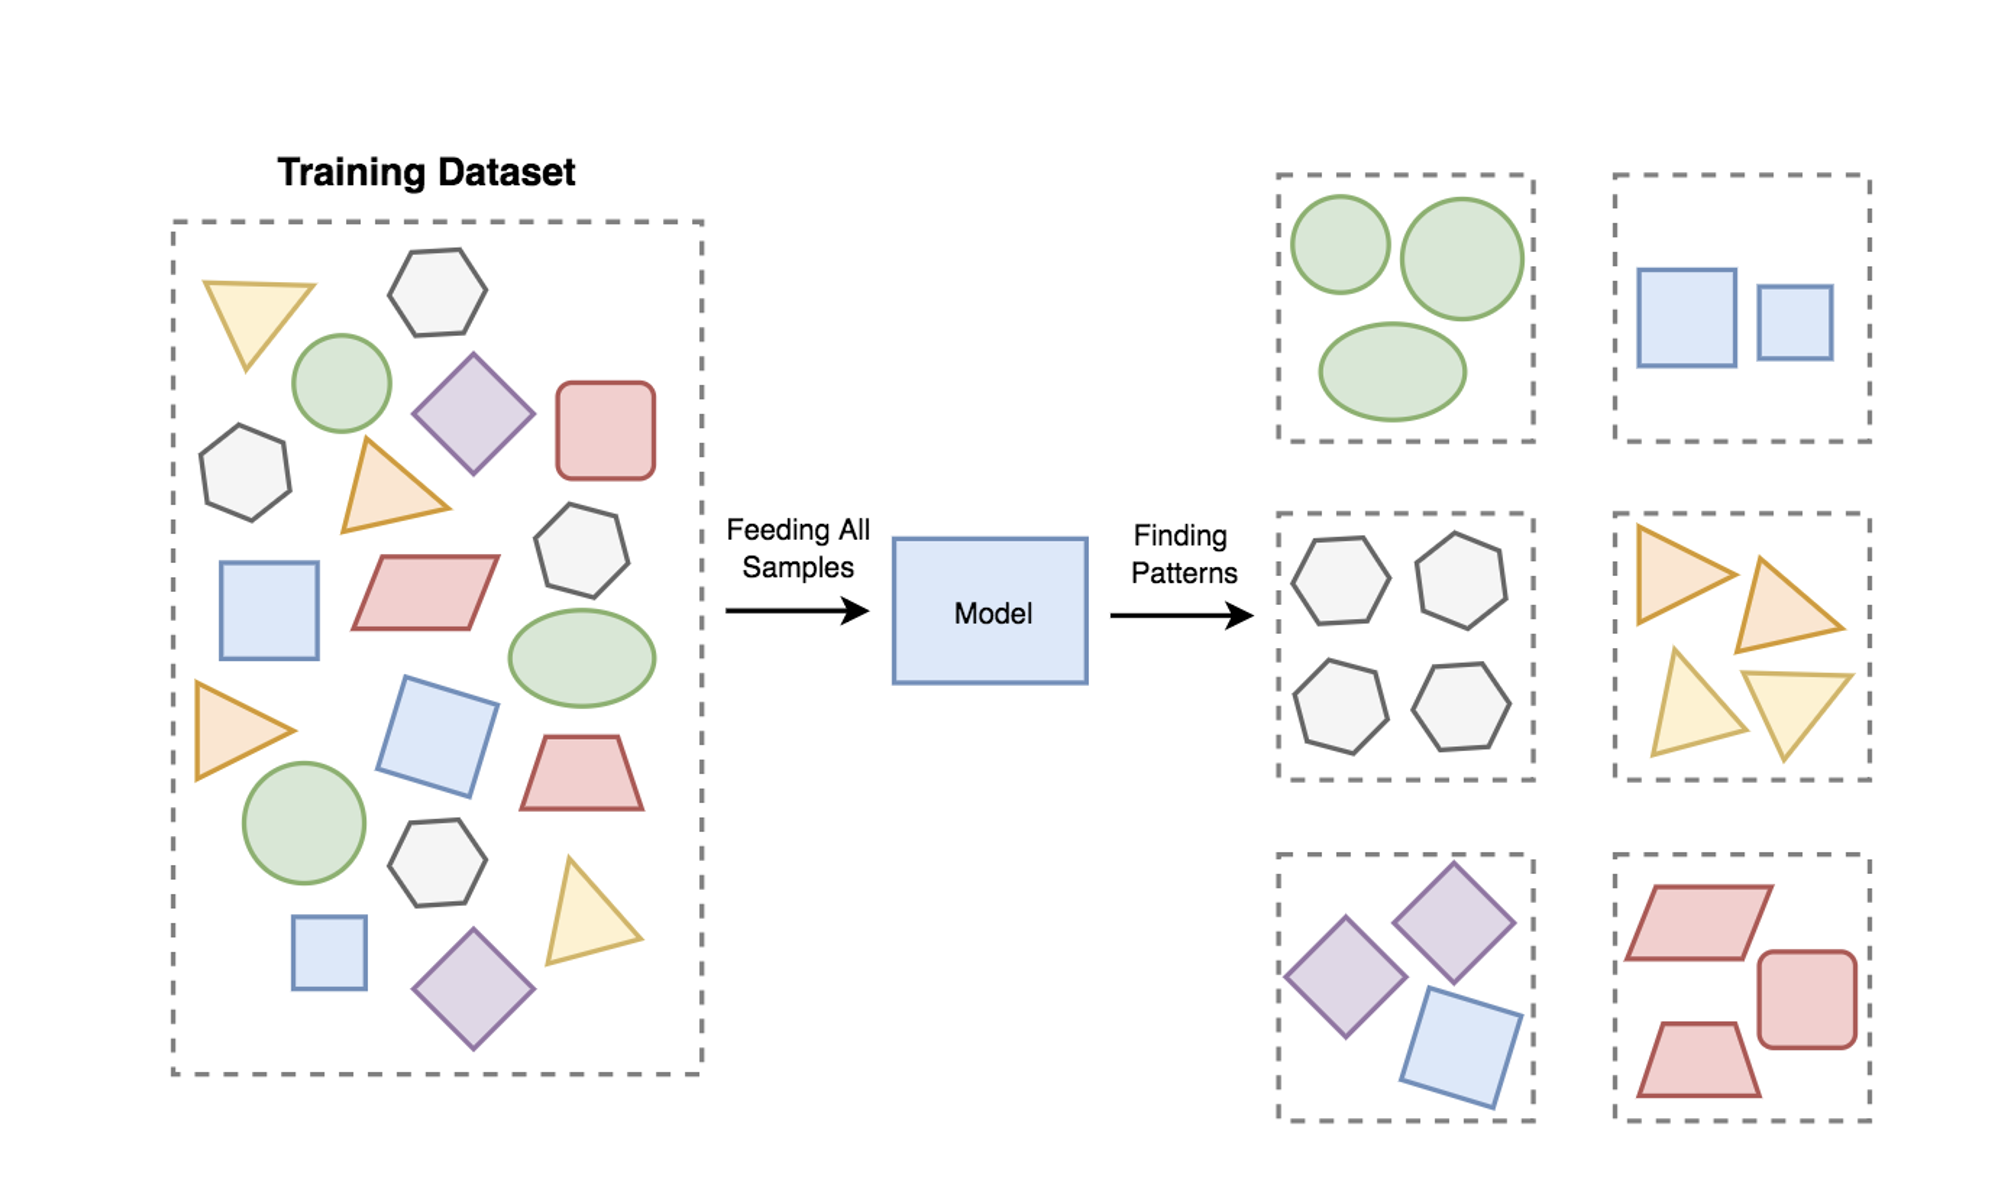
\includegraphics[width=1\linewidth]{img/page 3}
\end{frame}

\begin{frame}{Clustering v.s. Classification}
\protect\hypertarget{clustering-v.s.-classification}{}
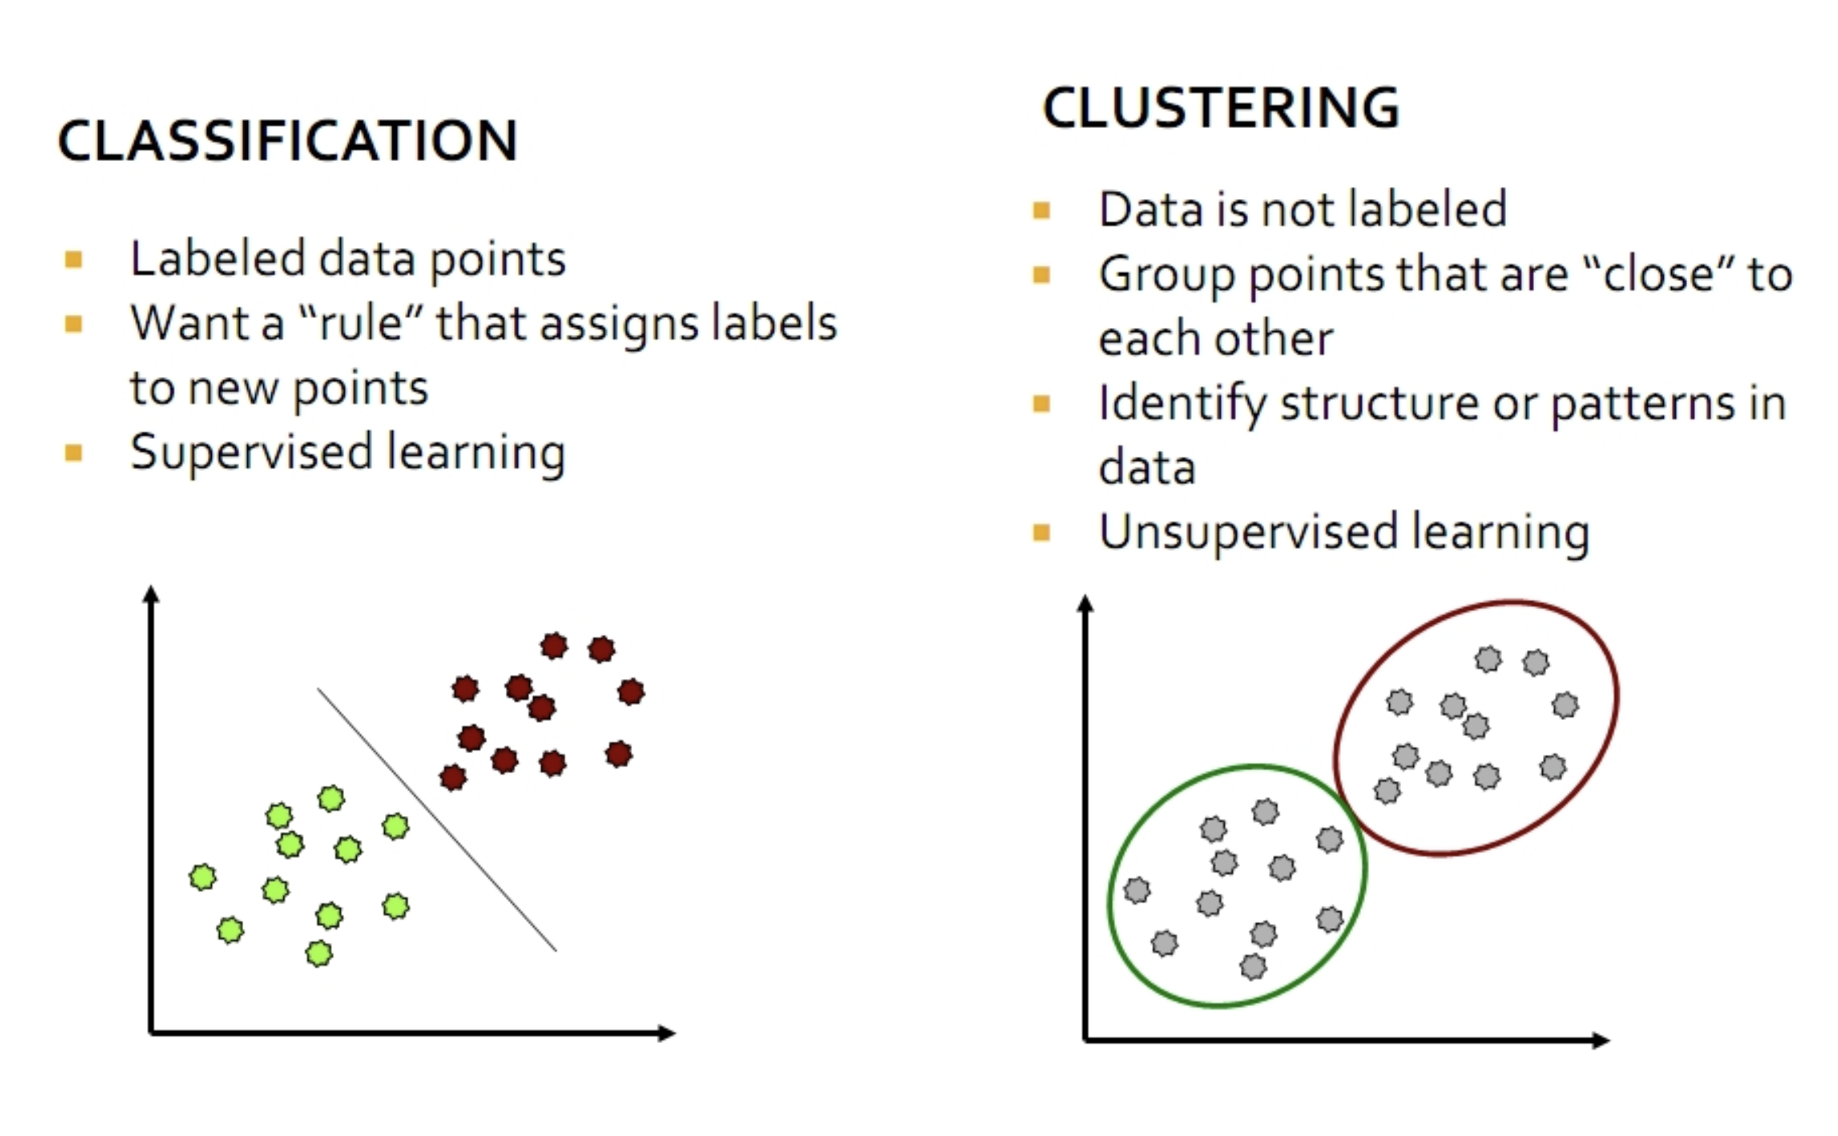
\includegraphics[width=1\linewidth]{img/page 4}
\end{frame}

\begin{frame}{Clustering}
\protect\hypertarget{clustering}{}
\begin{itemize}
\item
  Discover ``natural structure'' of data

  \begin{itemize}
  \tightlist
  \item
    What is the criterion?
  \item
    How to identify them?
  \item
    How to evaluate the results?
  \end{itemize}
\end{itemize}

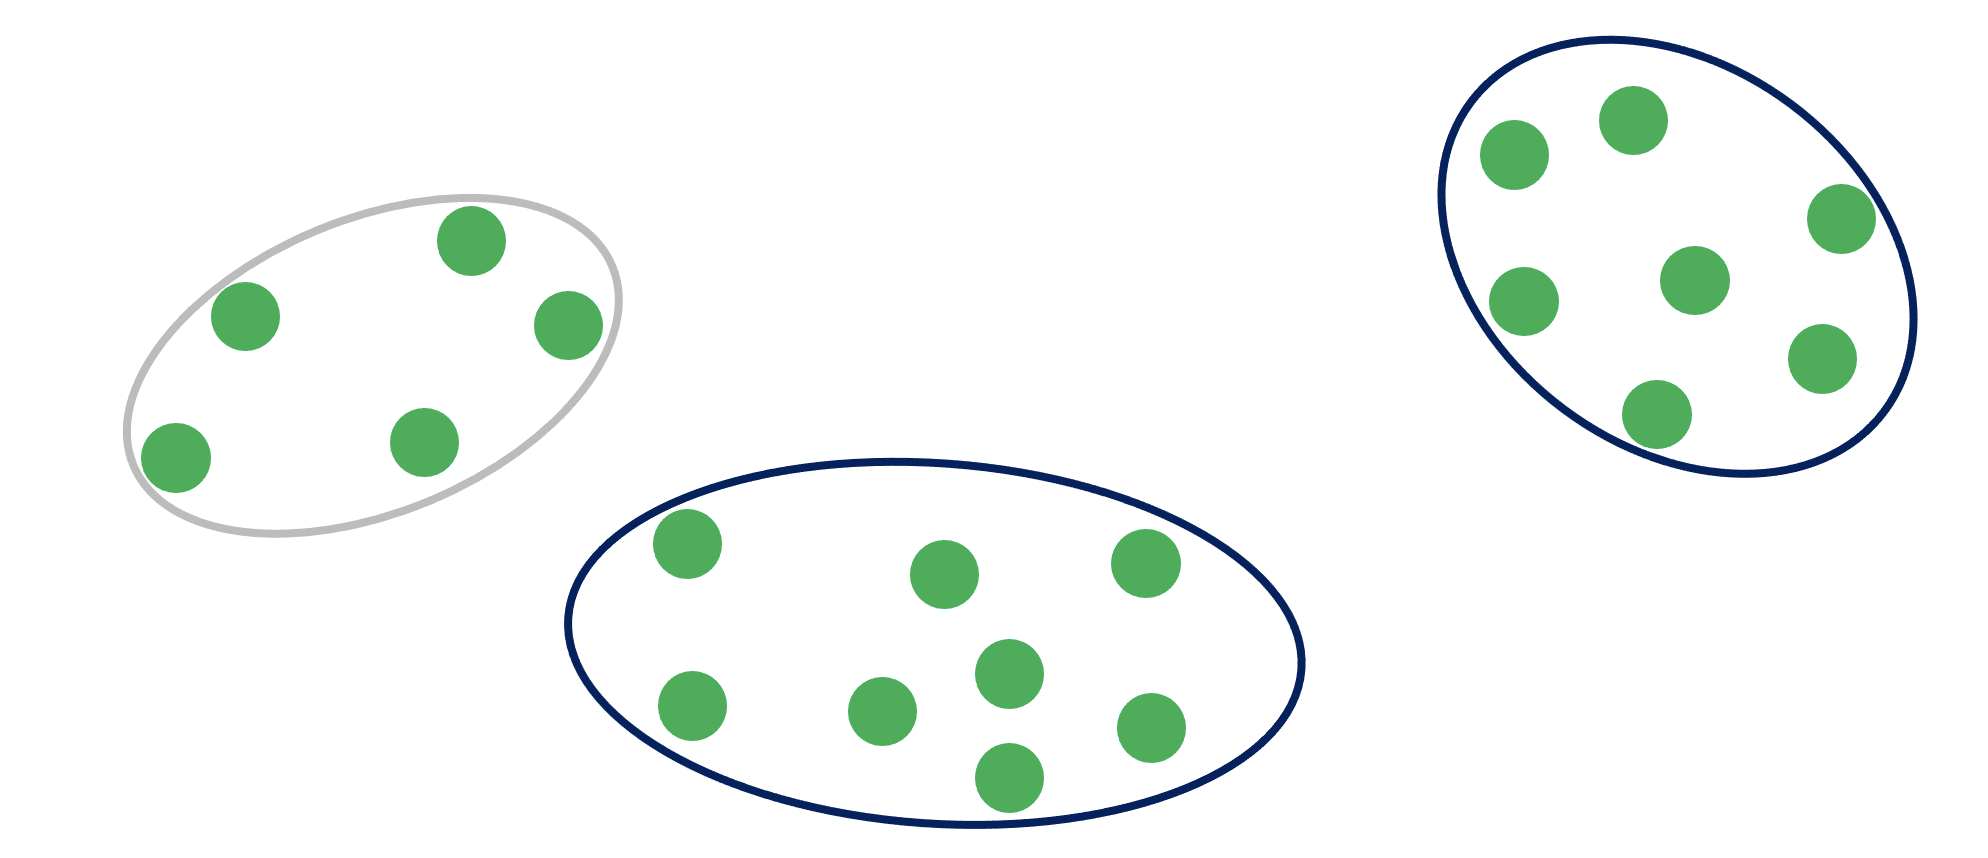
\includegraphics[width=1\linewidth]{img/page 5}
\end{frame}

\begin{frame}{Clustering}
\protect\hypertarget{clustering-1}{}
\begin{itemize}
\item
  Clustering - the process of grouping a set of objects into clusters of
  similar objects

  \begin{itemize}
  \item
    Basic criteria

    \begin{itemize}
    \item
      high intra-cluster similarity
    \item
      low inter-cluster similarity
    \end{itemize}
  \item
    No (little) supervision signal about the underlying clustering
    structure
  \item
    Need similarity/distance as guidance to form clusters
  \end{itemize}
\end{itemize}
\end{frame}

\begin{frame}{Applications of text clustering}
\protect\hypertarget{applications-of-text-clustering}{}
\begin{itemize}
\item
  Organize document collections

  \begin{itemize}
  \tightlist
  \item
    Automatically identify hierarchical/topical relation among documents
  \end{itemize}
\end{itemize}

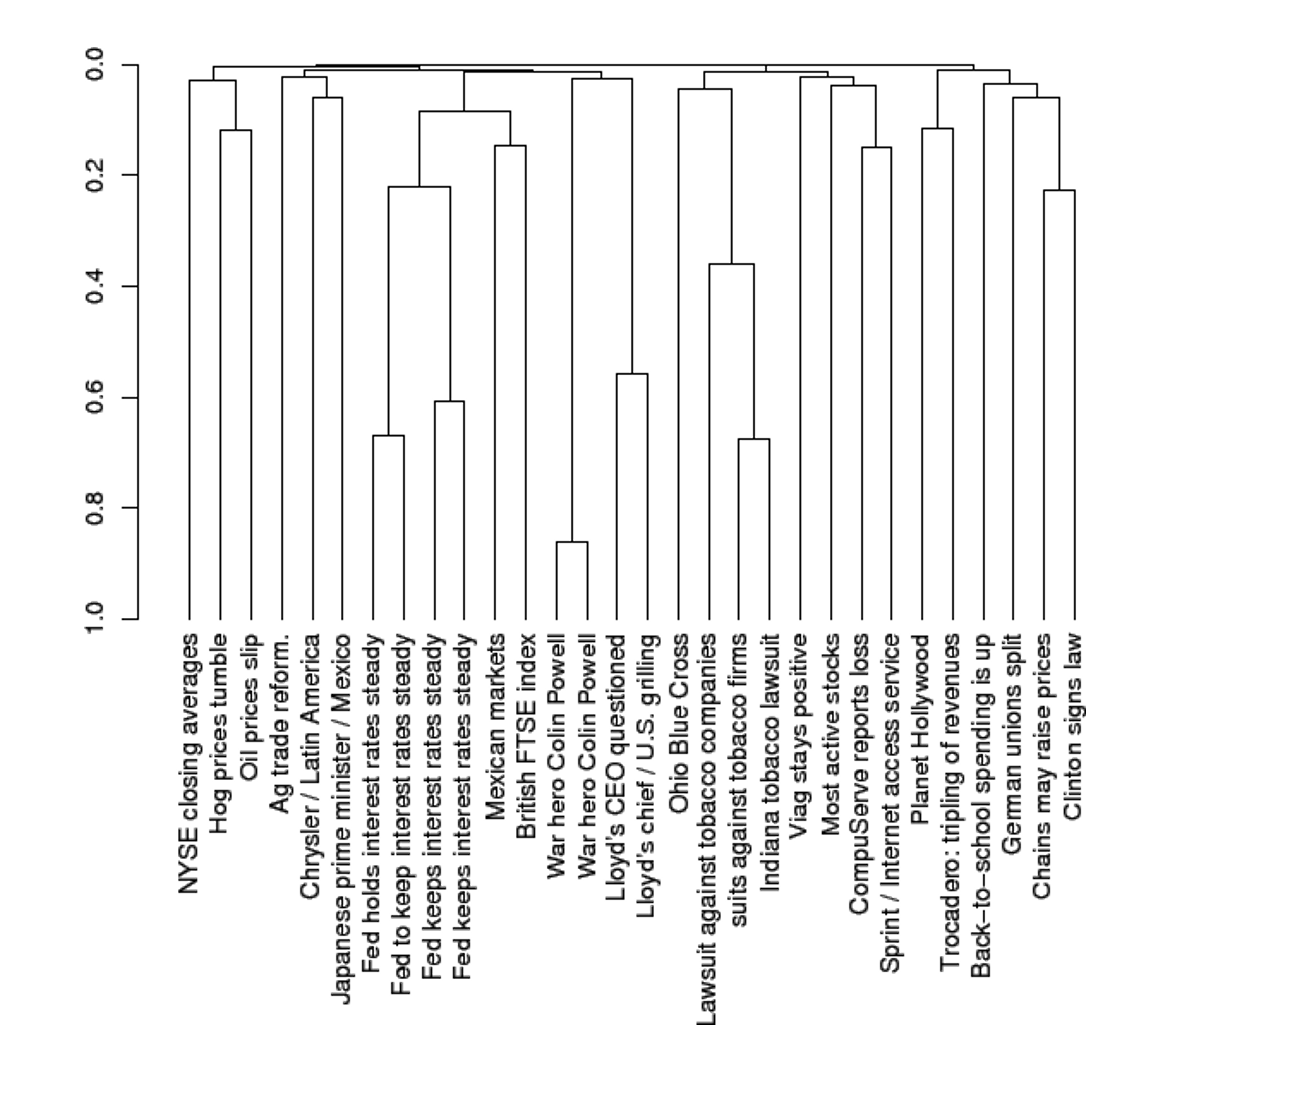
\includegraphics[width=1\linewidth]{img/page 7}
\end{frame}

\begin{frame}{Applications of text clustering}
\protect\hypertarget{applications-of-text-clustering-1}{}
\begin{itemize}
\item
  Grouping search results

  \begin{itemize}
  \item
    Organize documents by topics
  \item
    Facilitate user browsing
  \end{itemize}
\end{itemize}

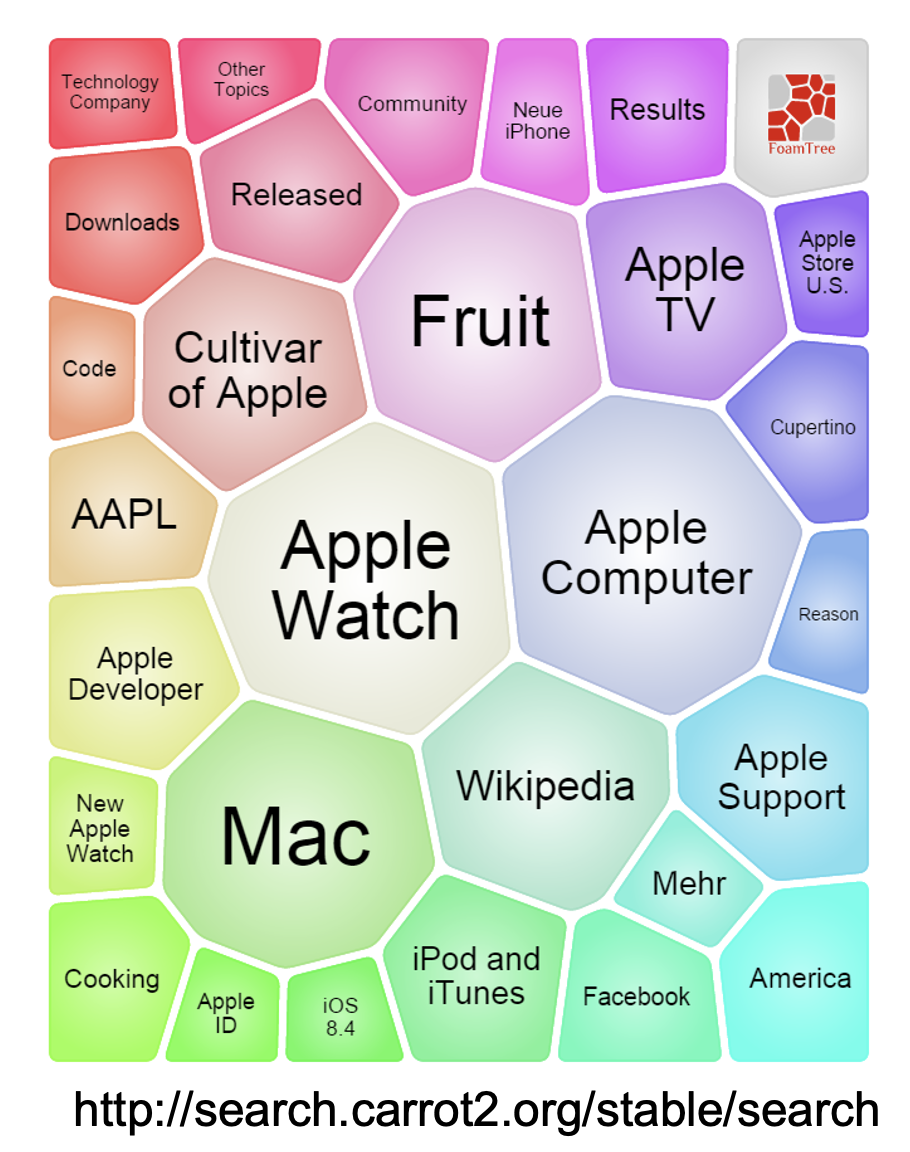
\includegraphics[width=1\linewidth]{img/page 8}
\end{frame}

\begin{frame}{Applications of text clustering}
\protect\hypertarget{applications-of-text-clustering-2}{}
\begin{itemize}
\tightlist
\item
  Topic modeling

  \begin{itemize}
  \tightlist
  \item
    Grouping words into topics
  \end{itemize}
\end{itemize}

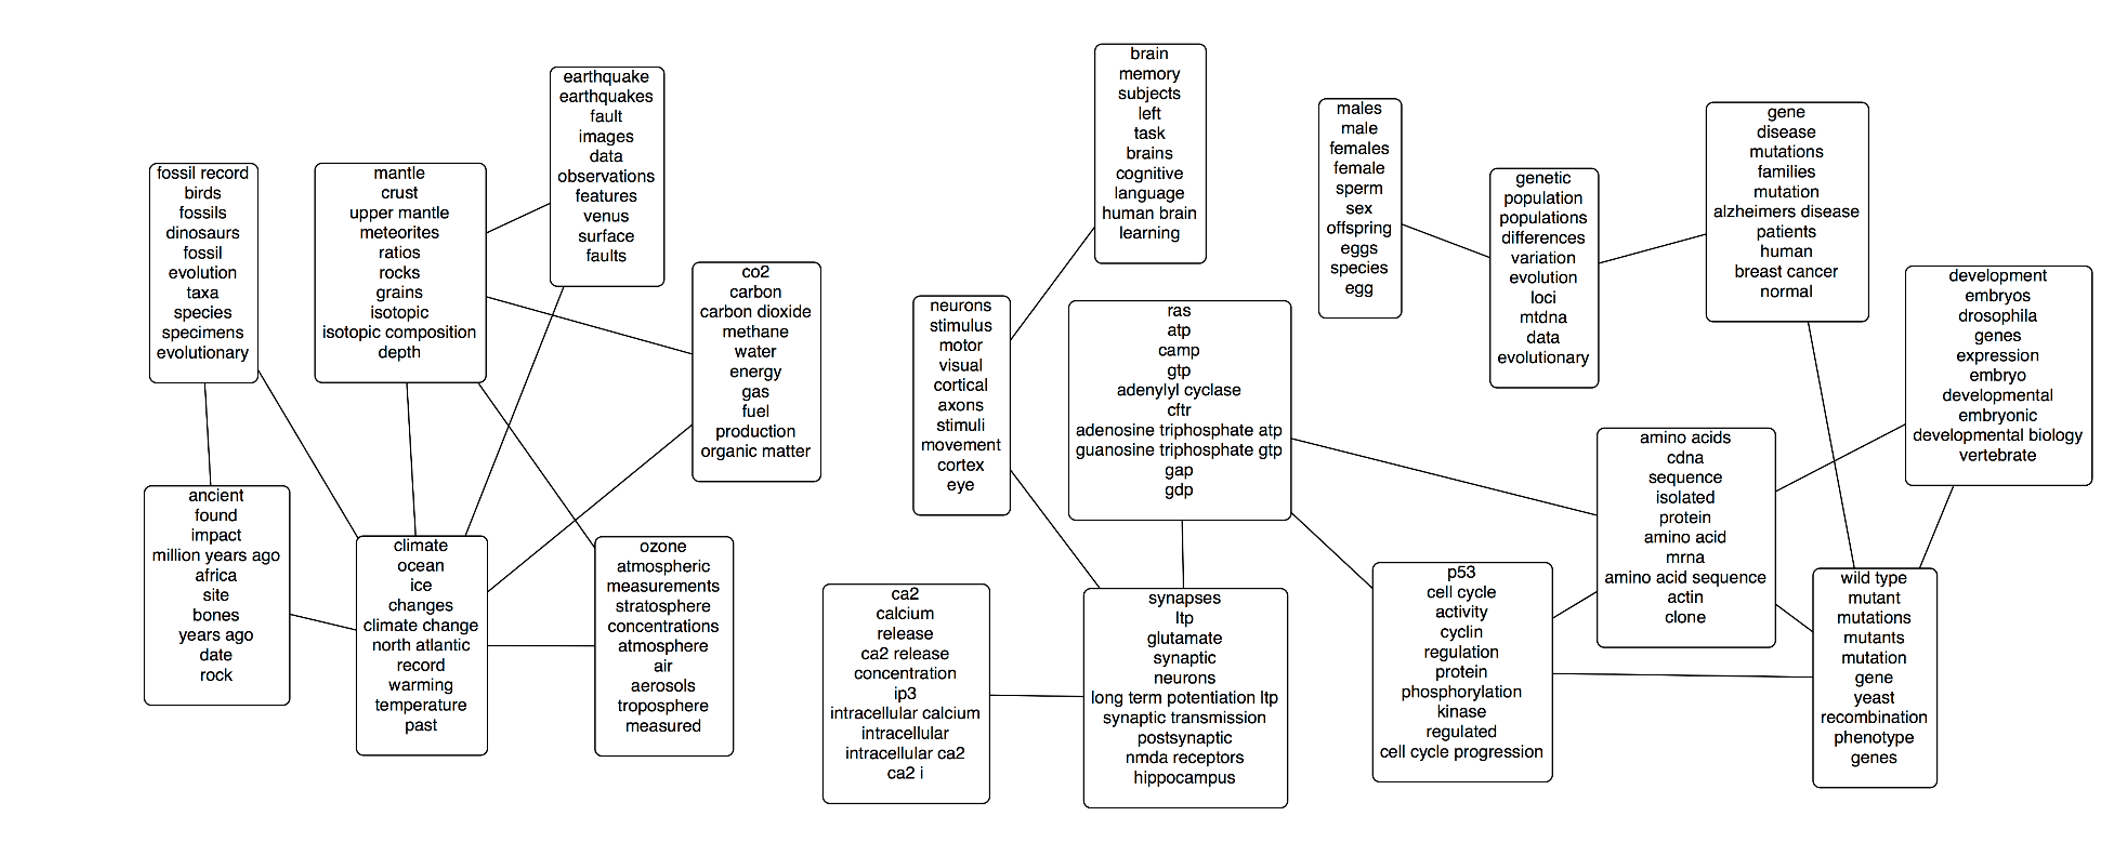
\includegraphics[width=1\linewidth]{img/page 9}
\end{frame}

\hypertarget{distance-metric}{%
\section{Distance metric}\label{distance-metric}}

\begin{frame}{Distance metric}
\protect\hypertarget{distance-metric-1}{}
\begin{itemize}
\item
  Basic properties

  \begin{itemize}
  \tightlist
  \item
    Positive separation

    \begin{itemize}
    \tightlist
    \item
      \(𝐷(x,y)>0, \forall x \neq y\)
    \item
      \(𝐷(x,y)=0, \mathrm{i.f.f.}, x=y\)
    \end{itemize}
  \item
    Symmetry

    \begin{itemize}
    \tightlist
    \item
      \(𝐷(x,y)=𝐷(y,x)\)
    \end{itemize}
  \item
    Triangle inequality

    \begin{itemize}
    \tightlist
    \item
      \(𝐷(x,y)≤𝐷(x,z)+𝐷(z,y)\)
    \end{itemize}
  \end{itemize}
\end{itemize}
\end{frame}

\begin{frame}{Typical distance metric}
\protect\hypertarget{typical-distance-metric}{}
\begin{itemize}
\item
  Minkowski metric

  \begin{itemize}
  \item
    \(d(x,y) = \sqrt[p]{\sum^V_{i=1}{(x_i-y_i)^p}}\)

    \begin{itemize}
    \tightlist
    \item
      When \(p=2\), it is {Euclidean distance}
    \end{itemize}
  \end{itemize}
\item
  Cosine metric

  \begin{itemize}
  \item
    \(𝑑(x,y)=1−cosine(x,y)\)

    \begin{itemize}
    \tightlist
    \item
      when \(|x|^2=|y|^2=1\), \(1−cosine(x,y)=\frac{r^2}{2}\)
    \end{itemize}
  \end{itemize}
\end{itemize}
\end{frame}

\begin{frame}{Typical distance metric}
\protect\hypertarget{typical-distance-metric-1}{}
\begin{itemize}
\item
  Edit distance

  \begin{itemize}
  \item
    Count the minimum number of operations required to transform one
    string into the other

    \begin{itemize}
    \tightlist
    \item
      Possible operations: insertion, deletion and replacement
    \end{itemize}
  \end{itemize}
\end{itemize}

\begin{flushright}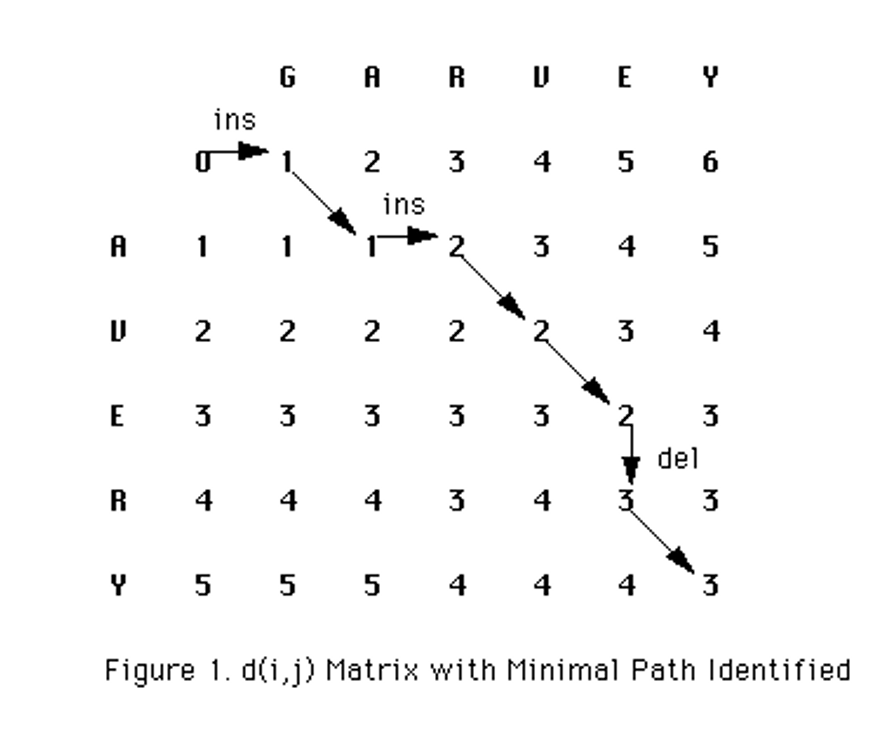
\includegraphics[width=0.7\linewidth]{img/page 13} \end{flushright}

← Can be efficiently solved by dynamic programming
\end{frame}

\begin{frame}{Typical distance metric}
\protect\hypertarget{typical-distance-metric-2}{}
\begin{itemize}
\item
  Edit distance

  \begin{itemize}
  \item
    Count the minimum number of operations required to transform one
    string into the other

    \begin{itemize}
    \tightlist
    \item
      Possible operations: insertion, deletion and replacement
    \end{itemize}
  \item
    Extent to distance between sentences

    \begin{itemize}
    \item
      Word similarity as cost of replacement

      \begin{itemize}
      \item
        ``terrible'' -\textgreater{} ``bad'': low cost {→ Lexicon or
        distributional semantics}
      \item
        ``terrible'' -\textgreater{} ``terrific'': high cost {→ Lexicon
        or distributional semantics}
      \end{itemize}
    \item
      Preserving word order in distance computation
    \end{itemize}
  \end{itemize}
\end{itemize}
\end{frame}

\hypertarget{clustering-algorithms}{%
\section{Clustering algorithms}\label{clustering-algorithms}}

\begin{frame}{Clustering algorithms}
\protect\hypertarget{clustering-algorithms-1}{}
\begin{enumerate}
\tightlist
\item
  Partitional clustering algorithms
\end{enumerate}

\begin{itemize}
\item
  Partition the instances into different groups
\item
  Flat structure

  \begin{itemize}
  \tightlist
  \item
    Need to specify the number of classes in advance
  \end{itemize}
\end{itemize}
\end{frame}

\begin{frame}{Clustering algorithms}
\protect\hypertarget{clustering-algorithms-2}{}
\begin{enumerate}
\setcounter{enumi}{1}
\tightlist
\item
  Hierarchical clustering algorithms
\end{enumerate}

\begin{itemize}
\item
  Create a hierarchical decomposition of objects
\item
  Rich internal structure

  \begin{itemize}
  \item
    No need to specify the number of clusters
  \item
    Can be used to organize objects
  \end{itemize}
\end{itemize}
\end{frame}

\end{document}
